\documentclass[a4paper,oneside]{book}

%% Language and font encodings
\usepackage[T1]{fontenc}
\usepackage[utf8]{inputenc}
\usepackage[italian]{babel}

%pacchetti
\usepackage{hyperref}
\usepackage{quoting}
\usepackage{graphicx}
\usepackage{booktabs}
\usepackage{caption}
\usepackage{array}
\usepackage{subfig} 
\usepackage{amsmath}
\usepackage{amsthm} 
\usepackage{amssymb}
\usepackage{mathtools}
\usepackage{braket}
\usepackage{empheq}
\usepackage{fancyvrb}
\usepackage{frontespizio}

%definizioni e teoremi
\theoremstyle{definition}
\newtheorem*{definizione}{Definizione}
\theoremstyle{plain}
\newtheorem*{teorema}{Teorema}

%Macro for \var
 \newcommand{\var}{\varphi} 


%% Setta page size e margini
\usepackage[a4paper,top=3cm,bottom=2cm,left=3cm,right=3cm,marginparwidth=1.75cm]{geometry}

\setlength{\parindent}{0pt}


\begin{document}


\includegraphics[scale=0.4]{ecmi-logo}

ECMI Modeling Week 2019\\
University of Grenoble - Grenoble INP

\begin{center}
\vspace{2.0cm}
{\Large{\textbf{THE TITLE OF THE PROJECT}}}

\vspace{\stretch{0.01}}

Instructor (University/Company)
\vspace{\stretch{0.01}}

\begin{tabular}{rl}
Author1 & (home university) \\
Author2 & (home university) \\
\ldots & \ldots \\
AuthorN & (home university)
\end{tabular}

\vspace{\stretch{0.5}}

Date of the report
\end{center}

\vspace{\stretch{0.15}}

% title page ends here

\newpage

\tableofcontents

% the actual thesis text starts here

\newpage







\chapter{A finite difference approximation for Schr{\"o}dinger equation}


We discretize our domain $\Omega=(a,b)$ with $N$ points and the uniform mesh is made by $N-1$ intervals of length $h=\frac{b-a}{N-1}$.

For the sake of simplicity we consider the a-dimensional time independent equation with \emph{transparent boundary conditions}, in $\Omega=(0,1)$, namely:


\[ \var''(x)+2(E-V(x))\var(x)=0 \]
 and conditions 
 \[ \bold{i} k \var(0)+\var'(0)=2\bold{i}k \] 
 
 \[ \var'(1)=\bold{i} k_2\var(1) \]


where $\bold{i}$ is the imaginary unit and $k_2=\sqrt{k^2+2(V(0)-V(1))}$, $k=\sqrt{2(E-V(0))}$.


Here $V:\mathbb{R} \rightarrow \mathbb{R}$ is the potential, which can be assumed to be piecewise constant. %% figure potential piecewise constant 
With the centered, second order, finite difference approach, the discretized equation becomes

 \[ \frac{\var_{i+1}-2\var_i +\var_{i-1}}{h^2}+2(E-V(x_i))\var_i=0, \quad i =1,\ldots, N\]


We can easily re-write the equation as a linear system using the fact that the part corresponding to the second derivative can be written as a \emph{matrix-vector} product $ A \cdot \boldsymbol{\var} $
where\[A= \frac{1}{h^2}
\begin{bmatrix}
-2& 1 & 0 & 0 & \dots & 0 \\
1 & -2 & 1 & 0 & \dots & 0 \\
0 & \ddots & \ddots & \ddots & \ddots & \vdots \\
\vdots & \ddots & \ddots & \ddots & \ddots & 0 \\
0 & \dots & 0 & 1 & -2 & 1 \\
0 & \dots & 0 & 0 & 1 & -2
\end{bmatrix} 
\]

and the boundary conditions has still to be imposed. The above tridiagonal matrix can be easily generated with the following MatLab command
\begin{verbatim}
A=toeplitz(sparse([1,1],[1,2],[-2,1]/(h^2),1,m))
\end{verbatim}

Looking at the other term of the equation, one can easily see that the whole equation becomes 

\[ (A+B) \boldsymbol{\var} = \bold{0}\]

where $(B)_{i,j}=2(E-V(x_i)) \delta_{i}^{j}$.




\section{Boundary conditions}

We write the first boundary condition by discretizing the first derivative with a second order approximation, by introducing a \emph{ghost node} (or virtual node) $x_0=x_1-h$.


\[ \bold{i} k \var(1)+ \frac{\var_2-\var_0}{2h}=2 \bold{i} k \]

Now, we compute $\var_0$ as a function of $\var_1, \var_2$, and we put it into the first line of the discretized system, which is 

\[ \frac{\var_2 - 2\var_1+\var_0(\var_1,\var_2)}{h^2}+ 2(E-V(x_1))\var_1=0\]


This leads to the following first line  

\[ \var_1 (\frac{2 \bold{i}k}{h^2}-\frac{2}{h^2}+2(E-V(x_1))) + \var_2 (\frac{2}{h^2})=\frac{4 \bold{i}k}{h}\]

This strategy preserves the second order of the numerical scheme. The very same argument applies to the other boundary condition. After these conditions we will end up with a RHS $\boldsymbol{b}$ which is zero everywhere except for the first component $\boldsymbol{b}(1)=\frac{ 4 \bold{i} k}{h}$.

Finally, the linear system to solve is 


\[
\frac{1}{h^2}
\begin{bmatrix}
2 \bold{i}k-2+2h^2(E-V(x_1)) & 2 & 0 & 0 & \dots & 0 \\
1 & -2 & 1 & 0 & \dots & 0 \\
0 & \ddots & \ddots & \ddots & \ddots & \vdots \\
\vdots & \ddots & \ddots & \ddots & \ddots & 0 \\
0 & \dots & 0 & 1 & -2 & 1 \\
0 & \dots & 0 & 0 & 2 & 2 h \bold{i} k_2 - 2 -2 h^2 (E-V(x_m))
\end{bmatrix} 
\cdot
\begin{bmatrix}
u_1 \\
u_2 \\
\vdots \\
\vdots \\
u_{m-1} \\
u_m
\end{bmatrix}
=
\begin{bmatrix}
\frac{4 \bold{i}k}{h} \\
0 \\
\vdots \\
\vdots \\
\vdots \\
0
\end{bmatrix}
\]

It's solved by using the default command \emph{backslash} in MatLab, which can easily handle complex arithmetic.


\section{Consistency of the scheme}

In order to show the consistency of the scheme, we insert the analytical solution $\var(x)$ in the numerical scheme.

 \[ \frac{\var(x_{i+1})-2\var(x_i)+\var(x_{i-1})}{h^2}+2(E-V(x_i))=0 \quad i=2, \ldots, N-1 \]

and, assuming $\var \in \mathcal{C}^{4}$, we expand in Taylor series about $x=x_i$

\[ \var ''(x_i)+2(E-V(x_i))+ \var^{(4)}(\xi) \frac{h^2}{12}+\mathcal{O}(h^4), \quad \xi \in (x_{i-1},x_i)\]

and since $\var(x)$ is the analytical solution what remains is just $ \var^{(4)}(\xi) \frac{h^2}{12}+\mathcal{O}(h^4), \quad \xi \in (x_{i-1},x_i)$

\section{Stability}
%http://profs.scienze.univr.it/~caliari/aa1819/equazioni_differenziali/dispense.pdf#subsection.12.2.7







\section{Order of convergence}
%inserisci grafico ordine e SPIEGA come ottenerlo

In order to show numerically the order of convergence, we compared the infinity norm of the difference between the analytical solution and the numerical one for a different number of grid points. The constants in the analytical solution has been computed by solving a linear system. 
As a potential we chose  $V(x)=50$, $ x \in (0,1)$. In the following logarithmic scaled plot we can appreciate the right order of convergence 
\begin{figure}[h]
	 \centering
	  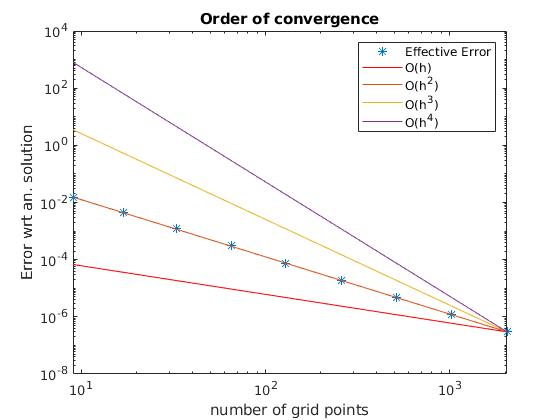
\includegraphics[width=0.8\textwidth]{OrderConst.jpg}
\end{figure}


\section{Possible improvement:  Galerkin approach}
%1-d FEM formulation. Pay attention to the boundaries

Since the regularity of $\var$ strongly depends on the regularity of the potential $V(x)$, with a finite difference approach one lose the second order approximation. Indeed, with piece-wise constant potential we have no more second order approximation. This observation leads to a Galerkin approach, requiring the solution $\var(x)$ to be less smooth than before. 

Denoting with $H^1(0,1)$ the Sobolev space $W^{1,2}(0,1)$, as usual we take a $v \in H^1(0,1)$, multiply the equations by $v$ and integrate by parts.

%
%\[
%\int_{0}^{1} \var ''(x) v(x)  \text{dx} + 2 \int_0^1 (E-V(x))\var (x) v(x) \text{dx} =0, \quad v \in H^1(0,1)
%\]



\[
[\var '(x) v(x)]_{0}^{1} - \int_{0}^{1} \var '(x) v'(x)  \text{dx}+ 2 \int_0^1 (E-V(x))\var (x) v(x) \text{dx} =0, \quad v \in H^1(0,1)
\]

Recalling that we have Robin boundary conditions, then in the weak formulation we will have terms proportional to $\var $. Using the fact that $\var'(0)=2 \bold{i} k - \bold{i} k \var(0)$ and $\var'(1)=\bold{i}k_2 \var(1)$ then the weak formulation is to find $u \in H^1(0,1)$ such that the following identity 

\[ 
\bold{i} k_2 \var(1)v(1) + \bold{i} k \var(0) v(0) -2 \bold{i}k - \int_0^1 \var' v' \text{dx} + 2 \int_0^1(E-V(x)) \var v \text{dx} = 2 \bold{i}k, 	\quad (\star)
\]

holds for every $v \in H^1(0,1)$

In order to solve it, we restrict to a proper finite dimensional subspace $X_h$ of $H^1$, made by piecewise linear functions, i.e. $X_h= \{ w \in H^1(0,1): w_{|[x_i,x_{i+1}]} \in \mathbb{P}([x_i,x_{i+1}])\}$. A basis of this space $X_h$ is given by the ``hat functions'' $w(x)$ and therefore we have to search for $\var_h \in X_h$ such that $(\star)$ holds for every $v \in X_h$. In particular, we have 

\[ 
\var_h(x)=\sum_{i=1}^{N} (\var_h)_j w_j(x)
\]

and the discrete problem is therefore to find $\var_h \in X_h$ s.t.

\[
-\int_0^1  \sum_j (\var_h)_j w_j'(x) w_i'(x) \text{dx} + 2 \int_0^1 (E-V(x)) \sum_j (\var_h)_j w_j(x) w_i(x) \text{dx} + \bold{i}k (\var_h)_1 w_{1}^{2}(0) + i k_2 (\var_h)_N w_n^{2}(1)= 2 \bold{i} k
\]

for $1\leq i \leq N$ 


\end{document}
